%http://svn.parisson.org/castax/
\chapter{L'acoustique}\label{Ch-Acous}
\begin{abstract}
En complément avec ce qui a été vu aux chapitres précédents~\ref{Ch-temps} et~\ref{Ch-ondes} sur les problèmes non stationnaires et les ondes, nous allons nous focaliser dans ce chapitre sur l'acoustique, et plus particulièrement sur le calcul de problèmes pour lesquels les fréquences restent inférieures à quelques milliers de Hz. Nous en profiterons pour effectuer une présentation pratique de l'acoustique et des solutions qui peuvent être mises en œuvre physiquement.
\end{abstract}

Nous avons déjà présenté la problématique de l'acoustique à plusieurs reprises au long de ce document: au paragraphe~\ref{Sec-EqOnde}, l'équation des ondes a été donnée dans le cas de l'acoustique sous forme d'équation différentielle~(\ref{Eq-EqOndeAcou}) dont l'inconnue est la pression acoustique; des remarques plus «physiques» concernant l'acoustique ont été faites au paragraphe~\ref{Sec-EqAcou}, notamment concernant les échelles d'énergies mises en œuvre, ainsi que sur les aspects solidien et aérien; mais c'est surtout au paragraphe~\ref{Sec-EqFblAcou} qu'ont été présentées l'équation d'Helmholtz~(\ref{Eq-Helm})\index[aut]{Helmholtz (Hermann Ludwig Ferdinand von -), 1821-1894, Allemand} et sa formulation faible. Quant à la formulation éléments finis, elle a été abordée au chapitre~\ref{Ch-ondes}, où ont été décrit les systèmes matriciels à traiter selon les cas (réponse libre, périodique ou transitoire, amortie ou non).

Toutefois, nous souhaitions apporter des éléments supplémentaires sur le sujet: 
\begin{itemize}
   \item au paragraphe~\ref{Sec-AcouPhy}, nous proposerons une présentation de l'acoustique «sur le terrain»: nous exposerons brièvement l'acoustique à partir des problématiques qui se posent physiquement, et nous présenterons quelques solutions typiquement utilisées pour résoudre ces problèmes d'acoustique. Nous verrons d'ailleurs que les problèmes rencontrés en hautes fréquences sont généralement aisément résolus, et qu'il convient donc de se concentrer sur les fréquences inférieures à 1000~Hz.
   \item au paragraphe suivant~\ref{Sec-AcouMEF} nous reviendrons plus en détails sur la mise en œuvre pratique d'un calcul acoustique par éléments finis.
   
   La motivation principale vient de ce que, dans le paragraphe~\ref{Sec-choc}, nous avons indiqué que la méthode des éléments finis devait se cantonner aux basses fréquences, celles-ci allant jusqu'à 600~Hz environ. Il est vrai qu'au-delà, de nombreuses autres méthodes existent... et nous avions profité de ce paragraphe pour les présenter.
Néanmoins, l'augmentation rapide des capacités des ordinateurs, fait qu'il est tout à fait raisonnable aujourd'hui de traiter des cas allant jusqu'à quelques milliers de Hz, disons 3000~Hz pour fixer les idées, à l'aide de la méthode des éléments finis. Cela permet de traiter la plupart des cas pratiques qui se posent à nous, puisque nous aurons vu auparavant qu'il est souvent inutile de monter plus haut en fréquence.
   
   \item Enfin, un exemple de calcul par éléments finis d'un problème acoustique sera donné pour clore ce chapitre d'illustration et de complément.
\end{itemize}

\medskip

\medskip
\section{L'acoustique physique}\label{Sec-AcouPhy}

Nous nous proposons d'étudier comment une nuisance vibroacoustique se propage depuis son émission jusqu'à sa réception.
La source pourra être mécanique, aéro- ou hydrodynamique... et pourra couvrir un très large spectre de fréquences, depuis les plus basses (excitation vibratoire, i.e. inférieure à environ 500~Hz), jusqu'aux plus hautes (excitation acoustique, depuis 500 jusqu'à environ 8000~Hz).
La propagation nécessitera de connaître le ou les modes de transmission (solidien, aérien) ainsi que l'environnement de transmission (champ ouvert ou fermé).
La réception quant à elle sera liée à la la perception, qui elle-même sera décrite de manière normative (niveau, puissance) ou sensorielle (psycho-acoustique...).

\medskip
\subsection{Émission}

Face à une problème vibroacoustique, on est amené à considérer les questions:
\begin{itemize}
   \item \textcolorblue{Localisation:} où est-ce que ça fait du bruit? Il s'agit de trouver, dans un ensemble qui peut être très complexe (par exemple un véhicule, un compresseur...), où sont les sources.
   \item \textcolorblue{Identification/Séparation:} là où ça fait du bruit, qu’est-ce qui fait du bruit exactement? De manière plus détaillée que la localisation, il peut être nécessaire, pour les sources identifiées, de déterminer la contribution de certaines de leurs parties ou sous-ensembles: selon la modélisation souhaitée, on pourra se contenter de dire que la source vibroacoustique dans un véhicule est le moteur, où alors souhaiter s'intéresser plus finement aux injecteurs, au carter, à la boîte de vitesse...
   \item \textcolorblue{Enregistrement/Caractérisation:} quel bruit est émis par chaque source? Il s'agit de réaliser des enregistrements permettant de caractériser la source vibroacoustique considérée. Par exemple, un vibromètre laser permet de récupérer les vibrations (accélérations, vitesses), sans contact. De là, il est possible de re-synthétiser le son d'une seule pièce parmi un ensemble de pièces en fonctionnement. Les enregistrements permettent de caractériser la source en terme de spectre, puissance, directivité... et fournissent également des données utiles pour la restitution de résultats (par exemple données audio binaurales).
\end{itemize}

\medskip
La caractérisation des sources peut également déboucher sur des lois phénoménologiques, qui relient les caractéristiques vibro-acoustiques à certains paramètres tels que par exemple: le rapport de boîte, le régime moteur, le régime ventilateur...

\medskip
Notons enfin que lorsque l'on parle d'acoustique, la propagation finale se fait forcément dans l'air puisque c'est celle qui arrive jusqu'aux oreilles...

\medskip
\subsection{Transmission}

%\medskip
La figure~\ref{Fig-ondes} donne la répartition schématique des puissances (ou les différents types d'ondes à considérer).
\begin{wrapfigure}{l}{65mm}
\centering
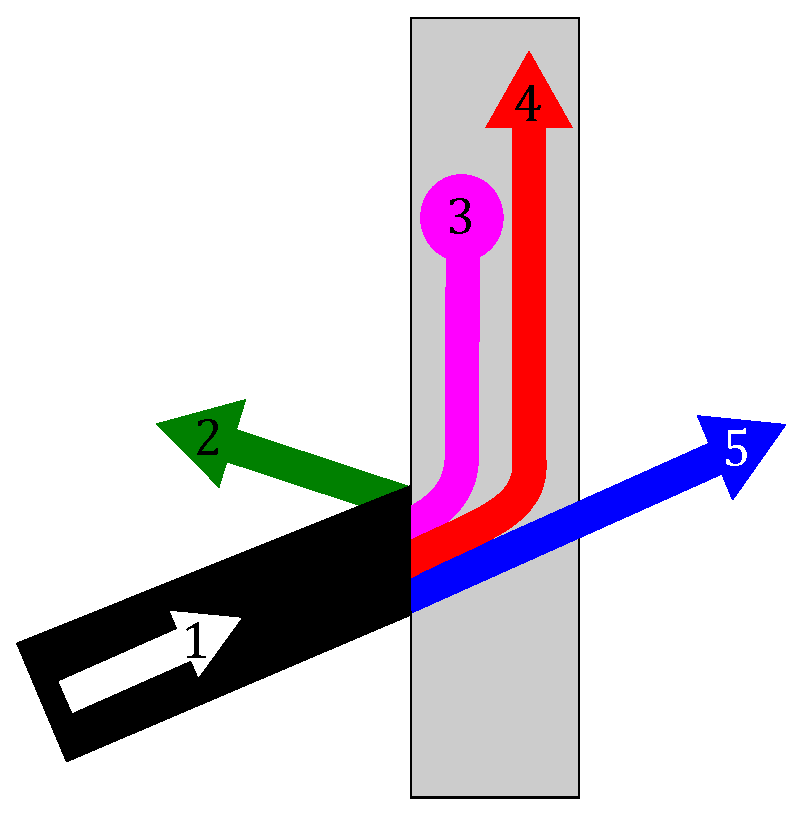
\includegraphics[height=55mm]{ondes.eps}\hspace{1cm}
\caption{Répartition schématique des puissances}\label{Fig-ondes}%: 1 = incidente, \textcolorgreen{2 = réfléchie}, \textcolormagenta{3 = absorbée}, \textcolorred{4 = propagée} et \textcolorblue{5= transmise}}
\end{wrapfigure}
Une onde incidente (1) arrivant sur un obstacle se trouve en partie \textcolorgreen{réfléchie par celui-ci (2)}, alors qu'une partie est directement \textcolorblue{transmise (5)}. Toutefois, cela ne représente pas la totalité de l'énergie incidente, car il reste encore une fraction qui est \textcolormagenta{absorbée ou dissipée par l'obstacle (3)}, et une dernière qui se \textcolorred{propage au sein de l'obstacle (4)} et qui peut ressurgir plus loin dans la structure considérée.

\medskip
Pour les matériaux acoustiques, la réflexion et la transmission seront déduites de mesures en tube d'impédance ou en cabine alpha, la capacité d'isolation sera caractérisée en utilisant la petite cabine, alors que la capacité de rayonnement sera appréhendée par le banc RTC III.

\medskip
L'\textcolorblue{isolement} est une donnée globale qui traduit la capacité d'un ensemble à «faire barrière au bruit». Il s'agit tout simplement de la différence entre ce qui attaque d'un côté et ce que l'on récupère de l'autre. Un isolement donné ne donne donc pas d'information sur la manière dont il est obtenu: réflexion, amortissement, absorption, ou plus probablement par une combinaison plus ou moins complexe (et inconnue) de ces trois phénomènes.

\medskip\newpage
Comme déjà mentionné au paragraphe~\ref{Sec-EqAcou}, il peut être nécessaire d'étudier un ou plusieurs des cas suivants:
\begin{itemize}
\item \textcolorblue{solidien/solidien:} la source excite mécaniquement la structure, et la vibration se propage dans la structure;
  \item \textcolorblue{aérien/aérien:} la source émet une vibration (un bruit) qui se propage dans l'air (en général). il s'agit de la propagation d'une onde acoustique de sa source jusqu'au récepteur, dans l'air;
  \item \textcolorblue{solidien/aérien:} il s'agit du cas du rayonnement. La source excite  mécaniquement une structure, et celle-ci ré-émet une onde dans l'air. 
  \item \textcolorblue{aérien/solidien:} dans le cas de sources acoustiques très puissantes, l'excitation acoustique se propageant dans l'air peut arriver à faire vibrer une structure.
\end{itemize}
Dans les deux premiers cas, on doit résoudre un problème de propagation dans un milieu (structure ou air). La sollicitation dépend du temps, donc on peut appliquer ce qui a été vu au chapitre~\ref{Ch-temps}; mais comme elle est généralement périodique, et que l'on s'intéresse au régime stationnaire, on peut alors utiliser ce qui a été vu au chapitre~\ref{Ch-ondes} sur les ondes.

Dans les deux derniers cas, il s'agit d'un calcul où il faut prendre en compte le couplage fluide-structure. La source étant périodique, on utilise encore ce qui a été vu au chapitre~\ref{Ch-ondes}, aussi bien dans la structure que dans l'air. Évidemment, ce sont les techniques du chapitre~\ref{Ch-temps} qui s'appliquent si l'on s'intéresse au régime transitoire.

\medskip
Dans la «réalité», tous ces cas existent bien:
\begin{itemize}
  \item solidien/solidien: tout moteur, même monté sur des silenblocs qui filtrent l'excitation, génère dans les supports, puis dans toute la structure porteuse, des vibrations. On est donc bien face à la propagation de vibrations au sein de solides;
  \item aérien/aérien: si l'on n'entre pas dans le détail de son fonctionnement mécanique, un haut-parleur est une source aérienne (en même une source ponctuelle, si l'on étudie par exemple une salle d'écoute, mais pas une source omnidirectionnelle) qui génère une onde acoustique qui se propage dans un volume d'air contenu, par exemple, dans une salle. Si l'on s'intéresse au niveau de pression acoustique en un point de la salle, on a une modélisation où seul le volume intérieur de la salle est nécessaire (et les bonnes conditions aux limites, mais nous y reviendrons);
    \item solidien/aérien: dans le cas de structures en treillis portant des panneaux, ce qui est le cas pour la conception de cars et bus, le moteur, situé à l'arrière, excite la structure de manière solidienne... et des vibrations se propagent dans tout le bus, où elles trouvent régulièrement, et jusqu'à l'avant, des panneaux qui vont se mettre à rayonner, i.e. à transformer cette vibration mécanique en bruit se propageant dans l'air jusqu'aux oreilles du conducteur et des passagers;
  \item aérien/solidien: dans le cas de structures légères, par exemple pour des véhicules sans permis, le moteur excite la structure non seulement de manière solidienne, mais également de manière aérienne. Le bruit généré par le moteur est tel, au sein du compartiment moteur, que cette sollicitation aérienne est capable de faire vibrer le tablier de séparation moteur/habitacle, qui dans ce cas précis est généralement très peu isolant (typiquement en ABS thermoformé avec une épaisseur avant transformation d'environ 3~mm, donc une épaisseur, dans les endroits les plus déformés, de l'ordre du millimètre). Il suffit pour le mettre en évidence de remplacer le moteur par un haut parleur découplé du châssis et générant une pression acoustique équivalente à celle du moteur.  
\end{itemize}
Tous ces cas existent donc bien, et peuvent même se superposer. Il convient donc d'être prudent dans le choix de la modélisation la plus adaptée au problème étudié.

\medskip
Il en va de même dans l'utilisation de matériaux ou solutions acoustiques. Plusieurs phénomènes peuvent intervenir et se superposer:
\begin{itemize}
   \item \textcolorblue{absorption:} il s'agit du cas où l'énergie acoustique est dissipée dans ou par le matériau ou la solution. Pour les matériaux poreux ou fibreux, des modèles de fluides équivalent existent. Ils sont modélisés par des paramètres tels que la porosité, la tortuosité... dans le cas de résonateurs ou de foils absorbers, ce sont les caractéristiques du matériau constituant ceux-ci ainsi que leur géométrie qui déterminent leur performance d'absorption;
   \item \textcolorblue{isolation:} il s'agit du cas où l'on fait barrière au bruit. Les notions d'étanchéité et de masses sont prépondérantes.
   
   On commencera donc par éviter au maximum toutes les fuites acoustiques (tous les trous);

Ensuite, on pourra utiliser le fait que l'isolation est liée à la masse: on gagne 6~dB par doublement de masse (en fait $20\log_{10}2$).

Enfin, d'autres systèmes peuvent être utilisés. Parmi ceux-ci, le système «masse-ressort» constitue l'une des plus anciennes solutions pour améliorer l'isolation acoustique. Il s'agit de réaliser un système rudimentaire de double parois découplées. Lorsque la première paroi est attaquée par le bruit et les vibrations, la seconde réagit de manière découplée. On peut choisir le ressort et la masse pour «filtrer» les fréquences indésirables. Ce système présente par contre une fréquence de coupure pour laquelle l'isolation n'est pas améliorée, mais au contraire le phénomène est amplifié.
   
   \item \textcolorblue{amortissement:} il s'agit du cas où l'énergie vibratoire est dissipée dans un matériau choisi pour ses propriétés d'amortissement visqueux, ou par son mode de fixation (collage, montage en contrainte...).
\end{itemize}
L'ajout d'une pièces d'insonorisation, par exemple réalisée par thermocompression de matières fibreuses, sur une structure a pour effet d'augmenter l'absorption. Toutefois, cette pièce possède une masse, même faible, qui ajoute de l'isolation. De plus, son mode de fixation peut apporter de l'amortissement à la structure étudiée. Mais, si la pièce est montée sur une tôle, sa masse étant vraiment faible face à celle de la tôle, il n'est pas faux de ne pas prendre en compte son apport sur l'isolation. Si de plus elle est juste maintenue mécaniquement, il est également possible de négliger leur influence en terme d'amortissement.

\medskip
Revenons quelques instants sur l'\textcolorblue{absorption}, et plus particulièrement sur les performances d'absorptions des solutions existantes, qui sont illustrées sur la figure~\ref{Mtx-alpha}.
\begin{figure}[h!]
\centering
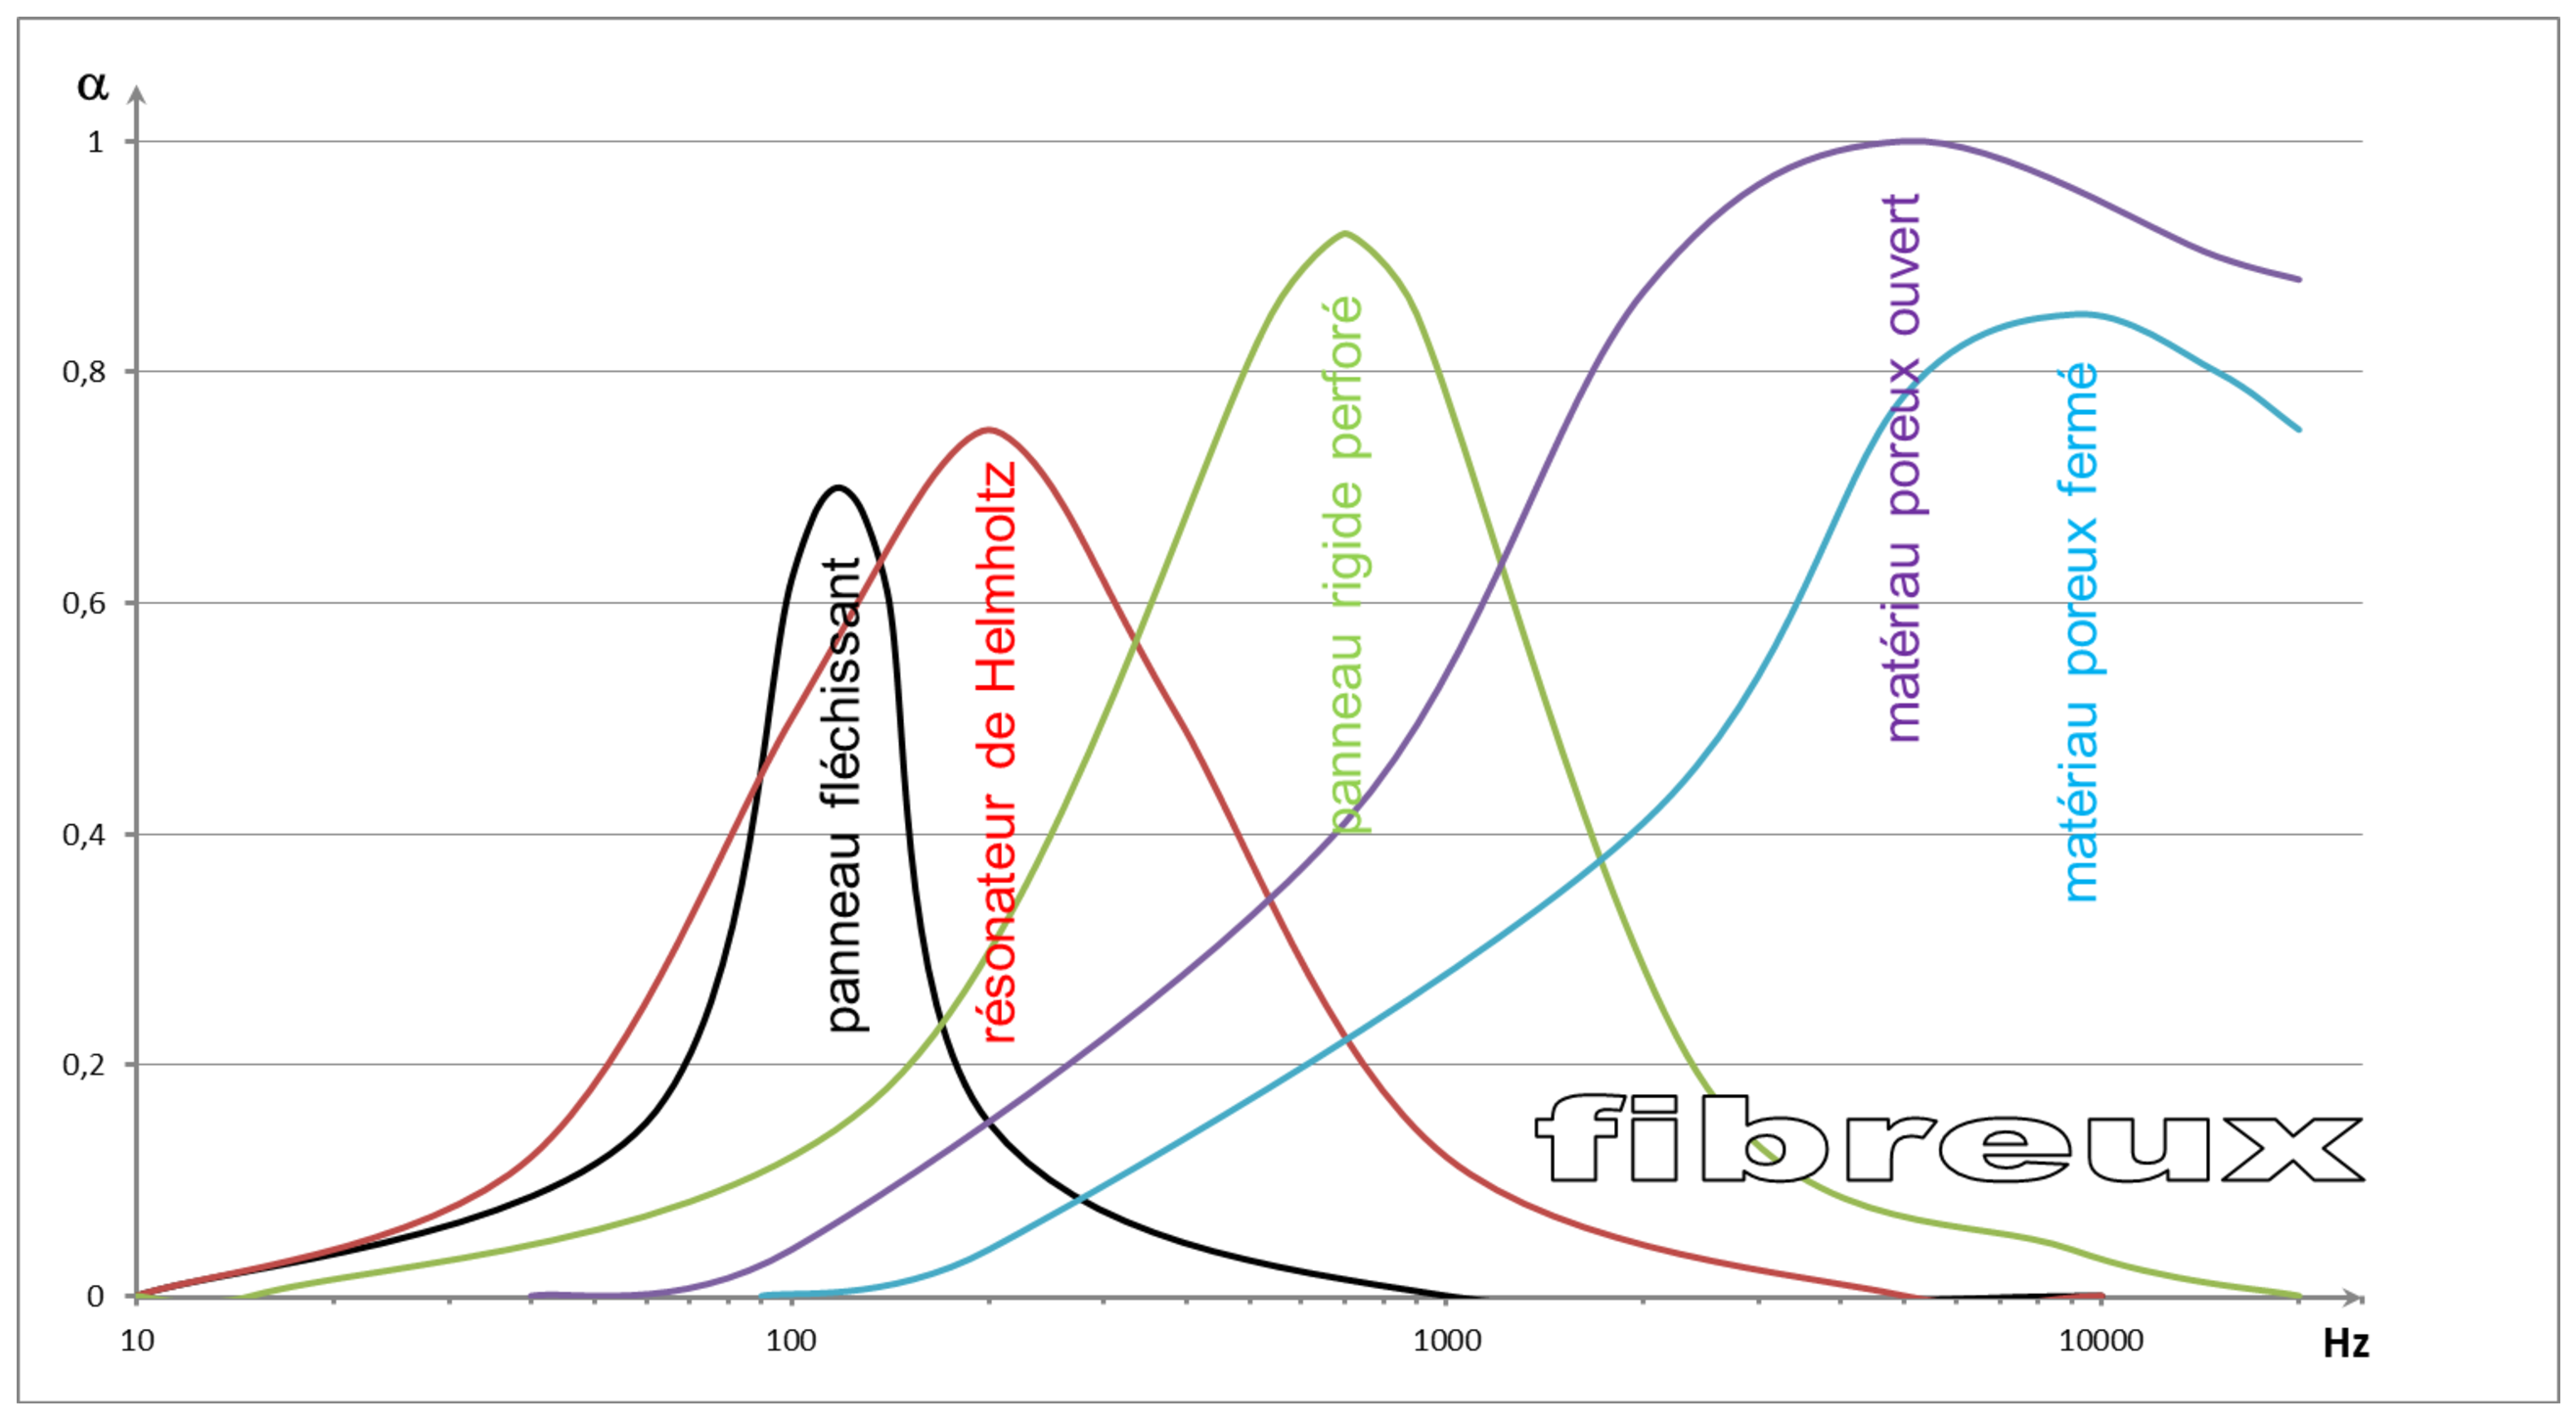
\includegraphics[width=150mm]{Mtx-alpha.eps}
\caption{Coefficient d'absorption pour différents types d'absorbants}\label{Fig-mtxalpha}
\end{figure}


\medskip
La \textcolorblue{diffraction} est un autre phénomène avec lequel il faut compter dans la propagation des ondes. Deux types apparaissent, comme illustré à la figure~\ref{Fig-diffrac}.
\begin{figure}[h!]
\centering
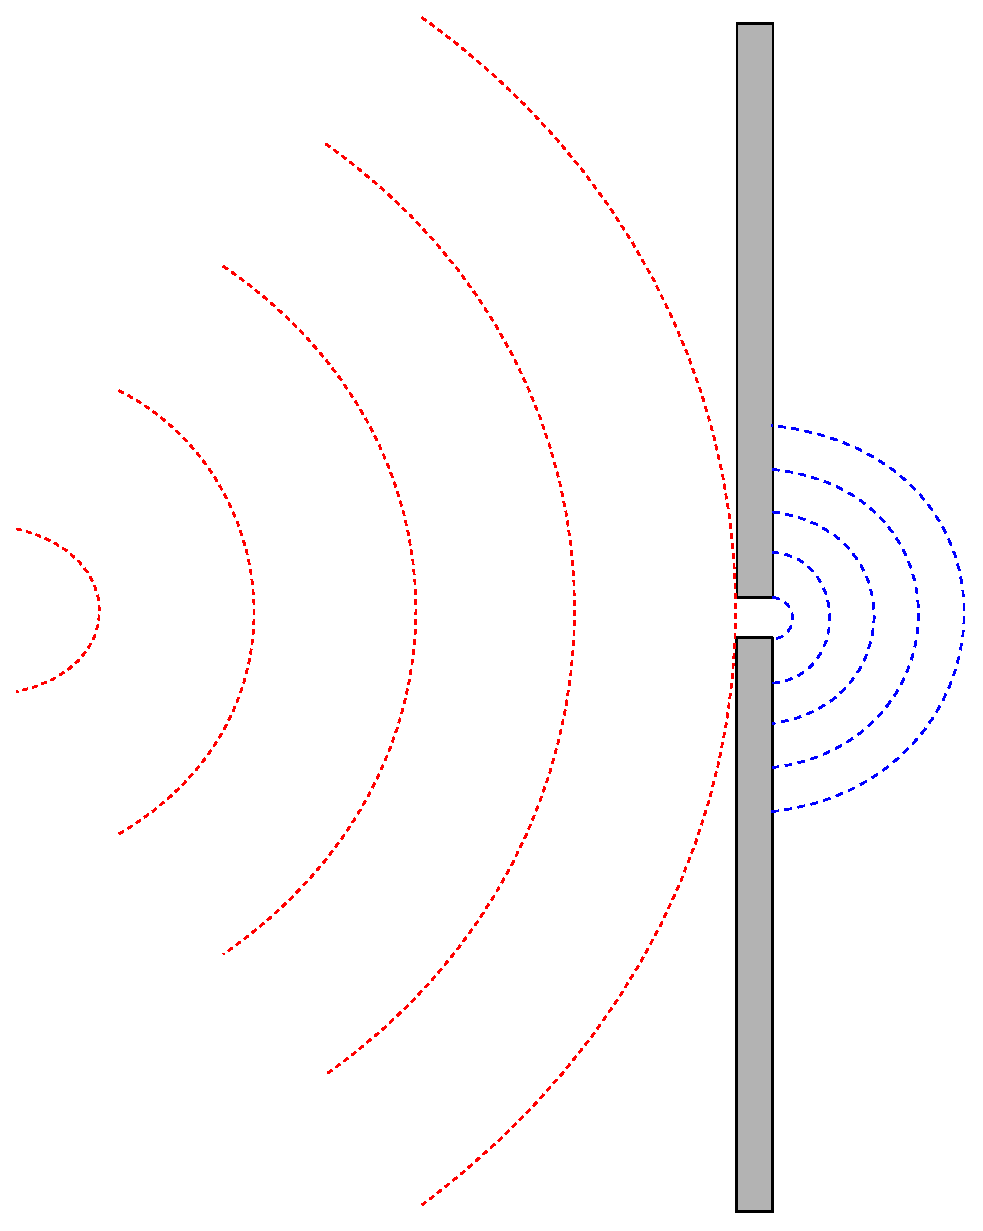
\includegraphics[width=40mm]{diffraction1.eps}\hfill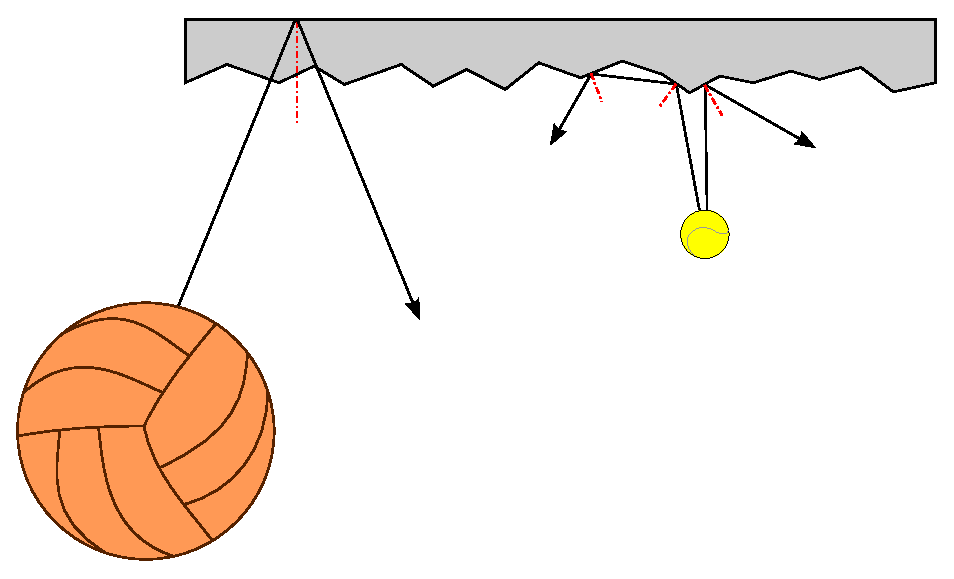
\includegraphics[width=60mm]{diffraction3.eps}\hfill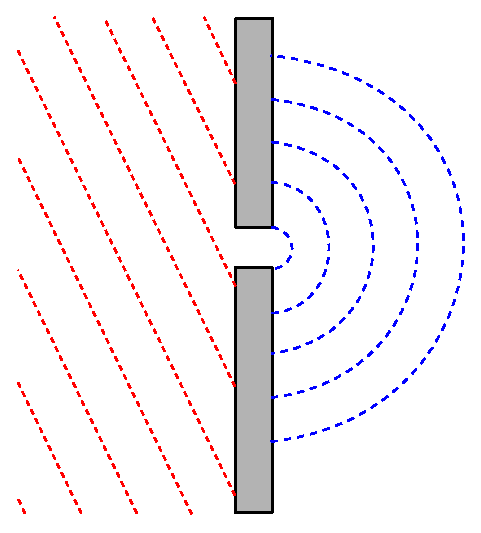
\includegraphics[width=32mm]{diffraction2.eps}
\caption{Phénomène de diffraction: a) au travers d'un trou, b) illustration avec des balles et c) réflexions sur un mur}\label{Fig-diffrac}
\end{figure}

Sur la figure~\ref{Fig-diffrac}a est représenté le phénomène de diffraction au travers d'une ouverture. l'onde après l'obstacle, i.e. l'onde diffractée, a la même fréquence, la même longueur d'onde et la même vitesse que l'onde incidente. Par contre, sa direction, son amplitude et sa forme sont modifiées (l'amplitude de l'onde diffractée  est inférieure à celle de l'onde incidente). C'est ce phénomène qui fait qu'au coin d'une rue, on entend la personne venant perpendiculairement à nous avant de la voir. Rappelons que deux ondes, diffractées ou non (mais ça a plus de sens ici en parlant d'ondes diffractées) peuvent interférer.
Le phénomène analogue se produit également lorsqu'un obstacle est inséré au sein d'un fluide. Les ondes doivent «éviter» l'obstacle, ce qui modifie notamment leur direction sur les bords de l'obstacle, et génère plus en aval de l'obstacle des figures d'interférence.

La figure~\ref{Fig-diffrac}b illustre avec des balles le phénomène également décrit par la figure~\ref{Fig-diffrac}c, i.e. le cas de la \textcolorblue{réflexion contre une surface irrégulière}. Si la balle est grosse face à la taille des irrégularités, i.e. si la longueur d'onde est plus grande que «celle des irrégularités» (ici on a un mur «en accordéon» ayant un motif répétitif de longueur~$l$), alors le trajet est insensible aux irrégularités de la surface: la normale prise en compte est celle de la surface sans irrégularités. Lorsque la dimension de la balle, i.e. la longueur d'onde de l'onde incidente, s'approche de la longueur caractéristique des irrégularités, alors il convient d'être prudent. Si~$\lambda<l$, alors on peut encore utiliser les lois de l'optique géométrique, mais on voit qu'il est alors nécessaire de disposer d'une discrétisation suffisamment fine pour décrire ces irrégularités. Il reste le cas problématique où~$\lambda=l$: dans ce cas, on a effectivement un phénomène de diffraction qu'il est souvent difficile de prendre en compte, sauf par des formulation particulières. Souvent, ce cas n'est clairement pas pris en compte.


\medskip
Enfin, un bonne question consiste à se demander ce qu'il se passe lorsqu'une source émet des fréquences qui «n'ont pas la place» de se développer au sein du volume disponible, i.e. \textcolorblue{lorsque les longueurs d'ondes considérées sont supérieures aux dimensions de l'espace dans lequel émet la source}. Ce cas se produit pour les basses fréquences émises par un moteur au sein de son encoffrement, ce dernier étant approximativement un cube de longueur 60~cm.

Et bien, dans ce cas, l'énergie injectée «gonfle» en quelque sorte l'encoffrement. Celui-ci est sollicité en pression... et répond évidemment selon ses modes propres.
Dans de nombreux cas (encoffrement moteur, habitacle de véhicule...), il est nécessaire de prendre en compte la réponse modale du volume dans lequel on définit le problème, car celle-ci influe sur la répartition du champ acoustique.
Le champ acoustique dans de telles situations (et dans d'autres) est non uniforme, i.e. a des valeurs très différentes d'un point à l'autre.
Ces deux aspects sont illustrés à la figure~\ref{Fig-modalVh}.
\begin{figure}[h!]
\centering
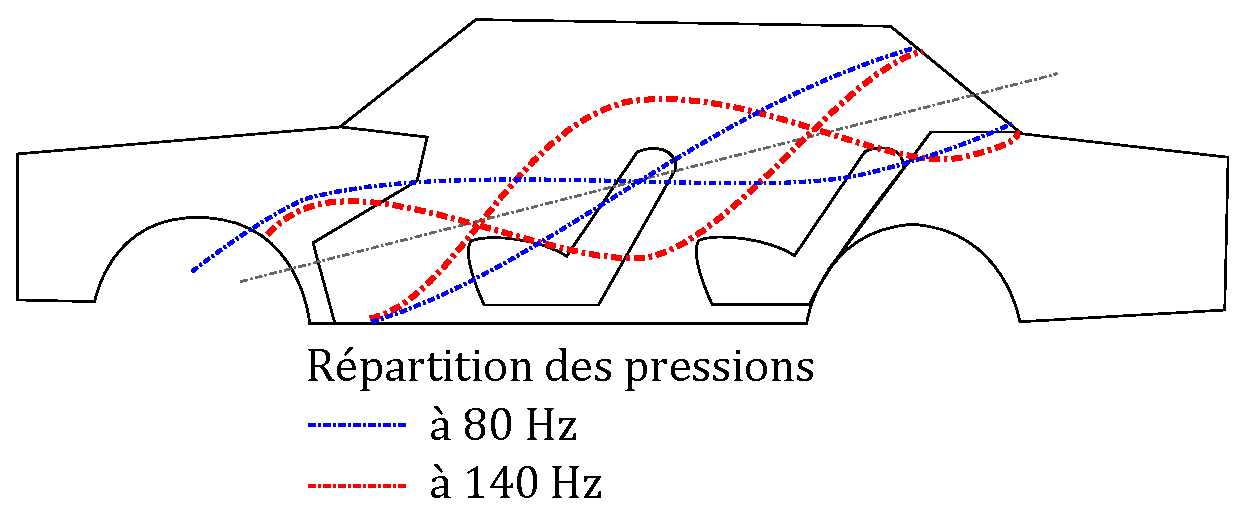
\includegraphics[width=95mm]{modalVh1.eps}\hfill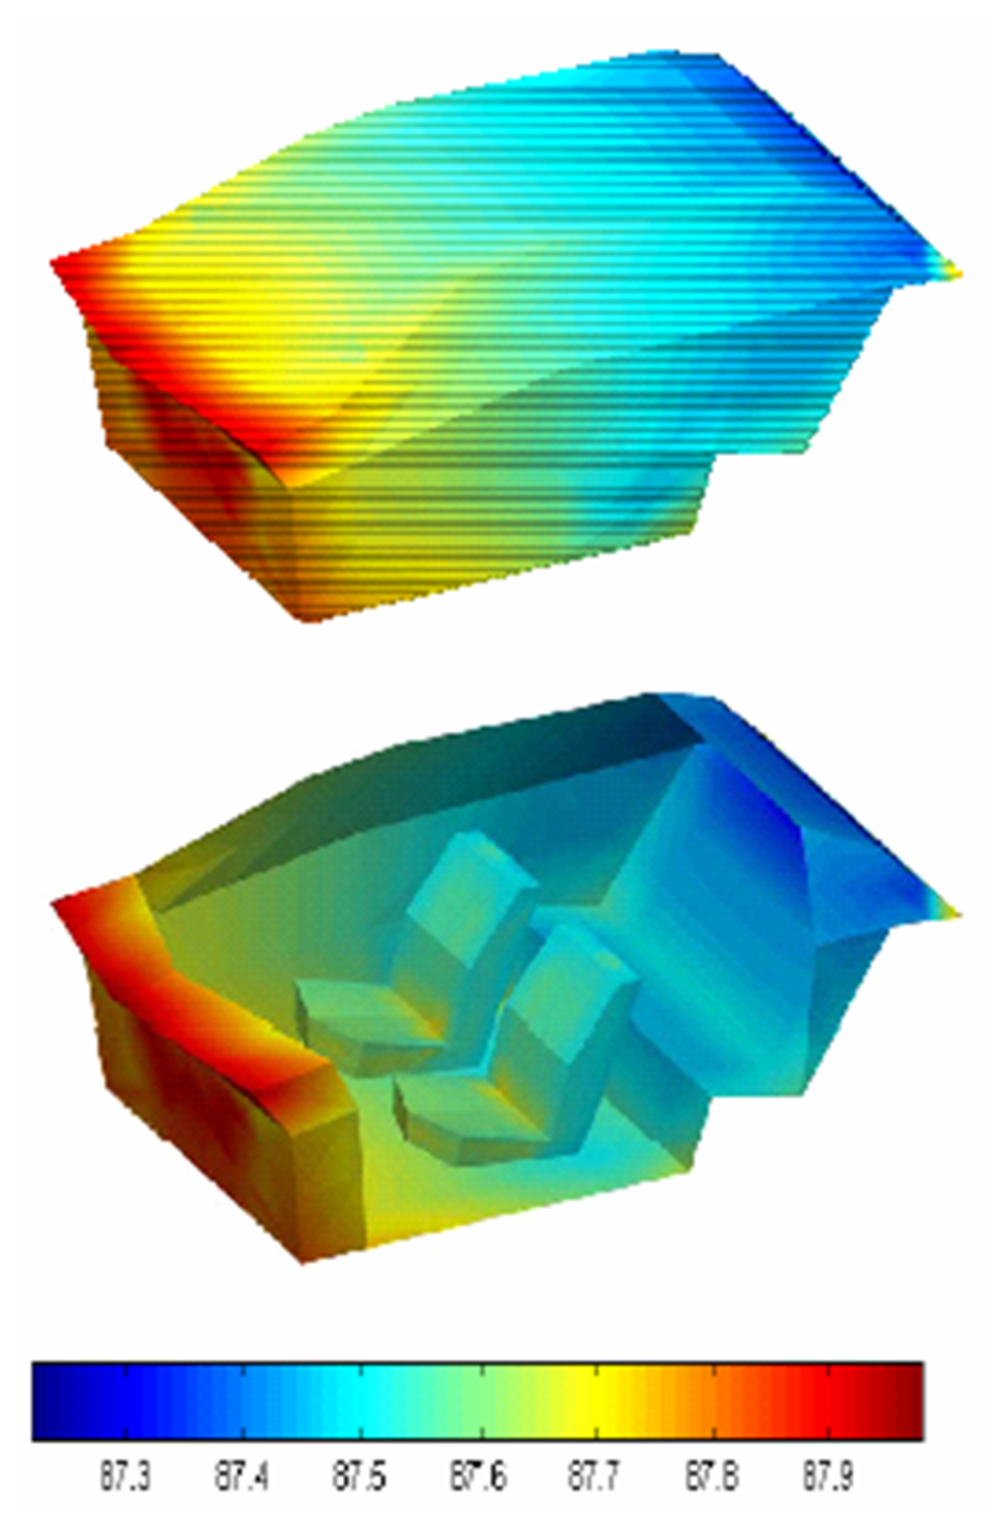
\includegraphics[height=55mm]{modalVh2.eps}
\caption{a) Répartition modale dans un véhicule et b) non-uniformité du champ acoustique}\label{Fig-modalVh}
\end{figure}

%hétérodynage

\medskip
\subsection{Réception}
%slides VM p27



\medskip
\section{Calcul acoustique par éléments finis}\label{Sec-AcouMEF}

\medskip
\subsection{Modélisation}

\medskip
\subsection{Condition CFL}

\medskip
\subsection{Absorption}

\medskip
\subsection{Vers l'infini...}
PML

\medskip
\subsection{... et au-delà}
Far Field


\medskip
\section{Exemple de calcul}


%\medskip
%\section{Un cas qui ne fonctionne pas}
% sous réserve de trouver un cas où une excitation à la fréquence f1
% conduit à une solution à la fréquence f2:
% via un composant mécanique: on sait modéliser, donc pas d'intérêt
% via un milieu très dispersif ? à essayer